% !TEX root = ../EntropicNumeric.tex

\subsection{Gradient Flows and Evolution of Densities}
\label{sec_applicationGF}

The basic framework of gradient flows has been briefly laid out in Section \ref{subsec_gradientflows}. This Section details the application of Algorithm \ref{algo_scaling_stabilized} for solving them.
As the transition from the measures formulation to the density formulation and further to the algorithm with pointwise optimality conditions was carefully detailed in Sections \ref{sec_appli_UOT} and \ref{sec_appli_bary}, we skip some of these intermediate steps here.

\subsubsection{In the Wasserstein Space}
Scaling algorithms for solving Wasserstein gradient flows are not new (see \cite{2015-Peyre-siims}), but our framework allows to simplify the derivation of the algorithm and the stabilized Algorithm \ref{algo_scaling_stabilized} allows to use much smaller regularization parameter $\epsilon$ yielding sharper and more precise flows. Given a convex, lower semicontinuous function on measures $\mathcal{G}$ with compact sublevel sets, each step requires to find the minimizer of
\eq{
\min_{\gamma \in \Mm_+(X\times X)} \langle c, \gamma\rangle + \iota_{\{=\}}(P^1_\# \gamma| \mu_k^\tau) + 2\, \tau \, \mathcal{G}(P^2_\# \gamma)
}
where $c :(x,y)\mapsto |y-x|^2$ is the quadratic cost. This directly fits in our framework by choosing $F_1(s) = \iota_{\{=\}}(s\, \d x| \mu_k^\tau)$ and $F_2(s) = 2 \, \tau \, \mathcal{G}(s\,\d x)$. 
%
\begin{example}
If the energy is given by the relative entropy $\mathcal{G}=\KLm(\cdot|p \, \d x)$ for some reference measure $p \, \d x$, then the proximal step for $F_2$ is given by 
\eq{
\prox^{\KL}_{\frac1\epsilon F_2}(q) = \argmin_{s : X \to \RR} \left( \epsilon \KL(s|q) + 2\tau \KL(s|p)\right) =q^\frac{\epsilon}{\epsilon+2\tau}\cdot p^\frac{2\tau}{\epsilon+2\tau}\, .
}
This problem is identical to an unbalanced transport problem where one of the marginal is fixed and the other is controlled by a $\KLm$ divergence. The difference is, that we want to solve a whole sequence of such problems, each time taking the second marginal of the optimal coupling and plugging it into the next problem as constraint for the first marginal. The gradient flow associated to this example allows to recover the heat flow when $p\,\d x$ is the Lebesgue measure on $X=\RR^d$.
\end{example}
%
\begin{example}
Some models of crowd motion with congestion \cite{roudneff2011handling} can be simulated by computing a sequence of measures $(\mu^\tau_{k})$ from an initial measure $\mu_0$, where for all $k\in \NN$, $\mu^\tau_{2k+1}$ is obtained from $\mu^\tau_{2k}$ by performing a free evolution during a time $\tau$ (this requires another algorithm) and then defining $\mu^\tau_{2k+2}$ as the Wasserstein projection of $\mu_{2k+1}^\tau$ (which we write as $p_{2k+1}\,\d x$) onto the set of measures with densities smaller than $1$. The second step can be performed by setting $F_1(s) = \iota_{\{=\}}(s|p_{2k+1})$ and $F_2(s)=\iota_{\leq 1}(s)$. The proximal operator of $F_2$ at a point $s$ is given by $\min \{1,s\}$ and thus $p_{2k+2}$ can be obtained from $p_{2k+1}$ with the stabilized Algorithm \ref{algo_scaling_stabilized} with 
\eq{
\proxdiv_{F_1}(s,u,\epsilon) = \tfrac{p_{2k+1}}{s}\,,
\qandq
\proxdiv_{F_2}(s,u,\epsilon) = \min \{\textstyle\frac1s , e^{-u/\epsilon}\}\, .
}
\end{example}

%%%%%%%%%%%%%%%%%%%%%%%%%%%%%%%%%%%%%%%%%%%%%%%%
\subsubsection[WF Gradient Flows]{$\WF$ Gradient Flows}
For $\WF$ gradient flows, each step requires to solve
\eq{
\inf_{\substack{\mu \in \Mm_+(X) \\ \gamma \in \Mm_+(X\times X)}} \langle c, \gamma \rangle + \KLm(P^1_\# \gamma | \mu_k^\tau) +  \KLm(P^2_\# \gamma | \mu) + 2 \tau \mathcal{G}(\mu)
}
where $c$ is the cost given in \eqref{logcost}. By denoting $p_k$ the density of $\mu_k^\tau$ with respect to $\d x$, one defines the functions
\eq{
F_1(s) = \KL(s|p_k) \qandq
F_2(s) = \inf_{p\in \Lun(X)} \KL(s|p) + 2\tau \, G(p)
}
where $G(p) \eqdef \mathcal{G}(p\d x)$.
%
If $G$ is an integral functional of the form $G(s) = \int_X g_x(s(x)) \d x$, the proximal operator is given pointwise by
\eq{
\inf_{(\tilde{s},p)\in \RR^2} \epsilon \KL(\tilde{s}|s)+ \KL(\tilde{s}|p) + 2\tau \, g_x(p)
}
for which the first order optimality conditions read
\eq{
\begin{cases}
0 = \epsilon \log (\tilde{s}/s) + \log(\tilde{s}/p) &\\
(\tilde{s}/p-1)/(2\tau)\in \partial g_x(p)
\end{cases}
}
and $\tilde{s}=0$ if $s=0$ or $p=0$. In many cases, this system can be easily solved, as in the following example.
% Example 1
\begin{example}
\label{exemple_GFtumor}
With the modelization of tumor growth in mind we introduce the functional 
\eq{
\mathcal{G}(\mu)=-\alpha \cdot \mu(X) + \iota_{\leq 1}({\d \mu}/{\d x})
}
where $\alpha \in ]0,\infty[$. This describes a model where cells have a tendency to multiply, but their density cannot exceed $1$. One can solve the time discretized gradient flow with Algorithm \ref{algo_scaling_stabilized} by choosing $F_2(s) =  \inf_{p} \KL(s|p) - 2\alpha\tau \, p + \iota_{\leq 1}(p)$. With the optimality conditions above, one obtains
%\eq{
%\prox^{\KL}_{\frac{1}{\epsilon}F_2}(s) = 
%\begin{cases}
%s\cdot (1-2\tau \alpha)^{-\frac{1}{\epsilon}} & \text{if $s\leq (1-2\tau \alpha)^\frac{1+\epsilon}{\epsilon}$} \\
%s^{\frac{\epsilon}{1+\epsilon}} &\text{otherwise.}
%\end{cases}
%}
\eq{
\proxdiv_{F_2}(s,u,\epsilon) = 
\begin{cases}
(e^u(1-2\tau\,\alpha))^{-\frac{1}{\epsilon}} & \text{if $s\leq e^{\frac{u}{\epsilon}}(1-2\tau \alpha)^\frac{1+\epsilon}{\epsilon}$} \\
(s\, e^u)^{-\frac{1}{1+\epsilon}} &\text{otherwise.}
\end{cases}
}
Moreover, given an optimal coupling $r$, one has $\mu_{k+1}^\tau = \min \left(\frac{P^2_\# r}{1-2\tau \alpha}, 1 \right)\d x$.
\end{example}
%
A numerical illustration is given in Figure \ref{fig_WFGF} where we used Algorithm \ref{algo_scaling_stabilized} (stopped after $500$ iterations) for solving each step , with the following parameters: $X$ is the segment $[0,1]$ discretized into $3000$ uniformly spaced samples, the initial density $p_0$ is the black line on Figure \ref{fig_WFGFprofile}, $\tau= 0.006$, $\alpha=1$ and $\epsilon = 10^{-8}$. The running time was $315$ seconds. Remark how, by using a very small value for $\epsilon$, the ``smoothing'' effect of the entropy disappears: the contours of the free-boundary which evolve with time remain sharp.

\begin{figure}
 \centering
\begin{subfigure}{1.\linewidth}
\centering
 \resizebox{1.\linewidth}{!}{
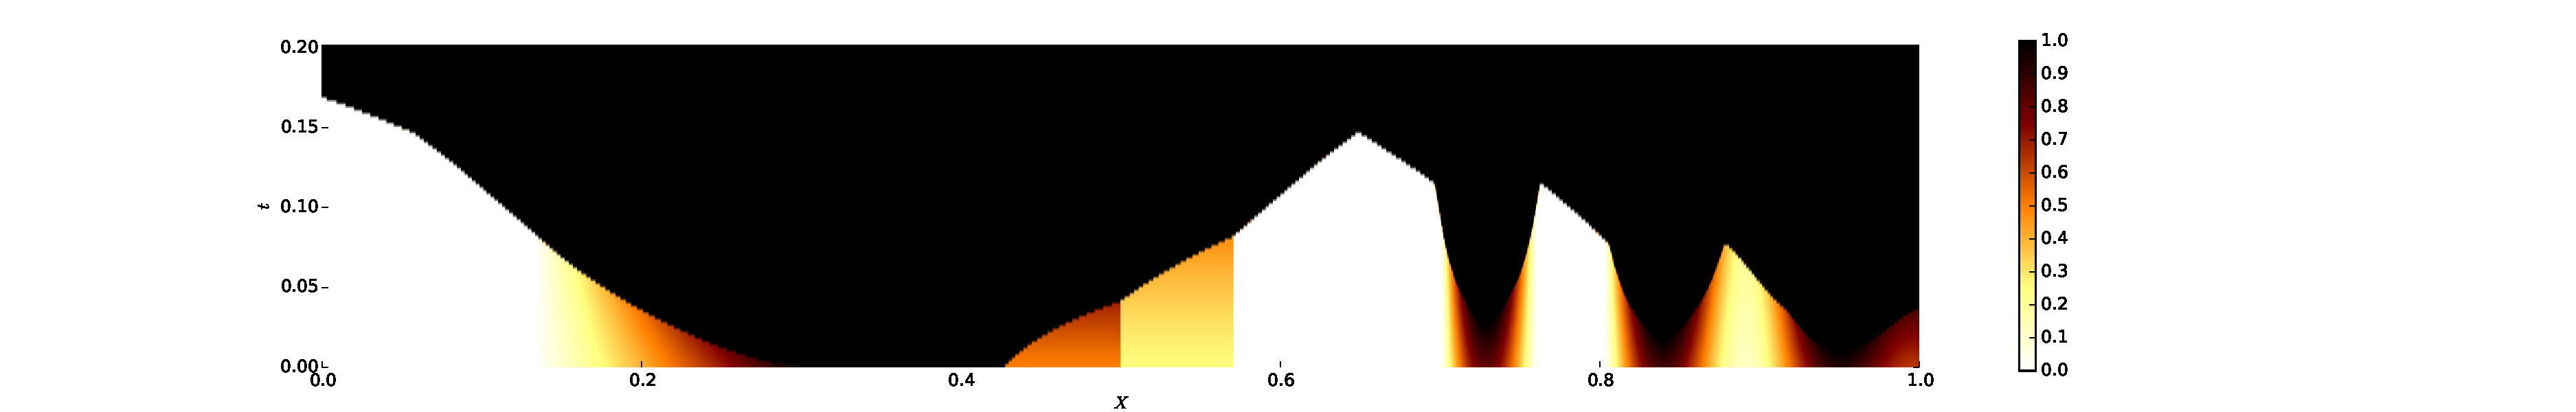
\includegraphics[clip,trim=-5cm 0cm 4.5cm 0cm]{GF/heleshaw1d_tophotbar}
}%
\caption{Evolution in color scale: time evolves from bottom to top.}\label{fig_WFGFtop}
\end{subfigure}
 \begin{subfigure}{.8\linewidth}
\centering
 \resizebox{1.\linewidth}{!}{
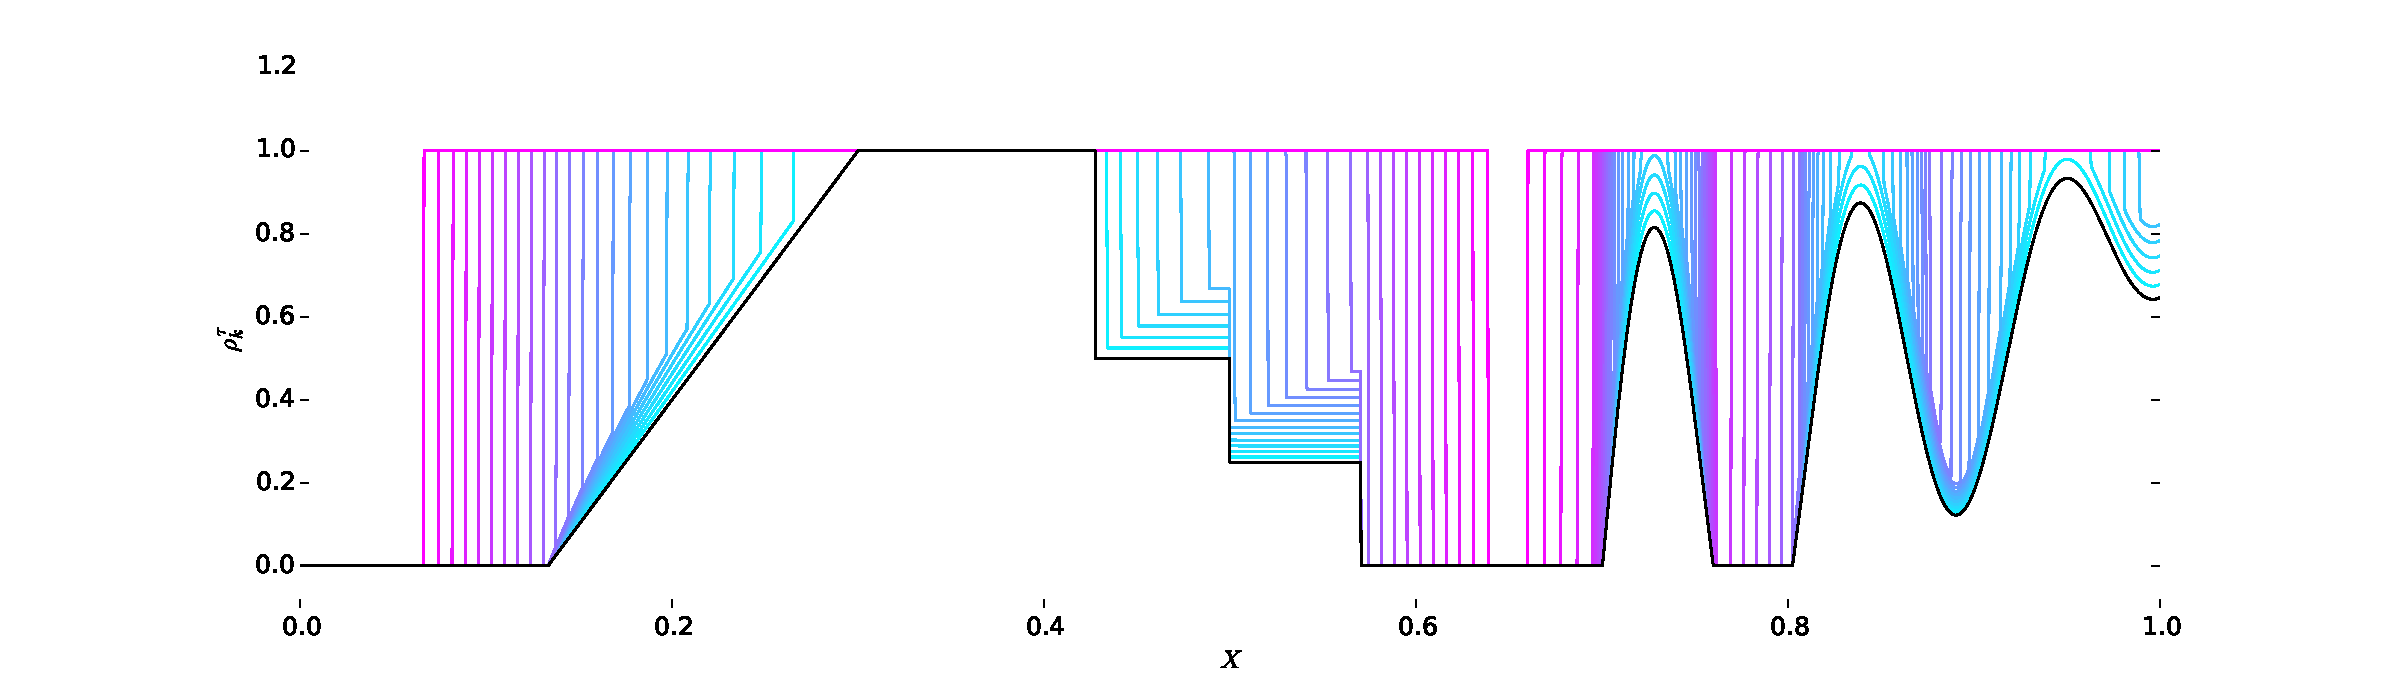
\includegraphics[clip,trim=0cm 0cm 0cm 0cm]{GF/heleshaw_profile}
}%
\caption{Evolution viewed ``laterally'' : the initial density $p_0$ is the black line, then the density is displayed at every time step with a color ranging from blue (small times) to pink (bigger times).}\label{fig_WFGFprofile}
\end{subfigure}
\caption{Evolution of the density with respect to time for the growth model of Example \ref{exemple_GFtumor}.}
\label{fig_WFGF}
\end{figure}


%
\subsubsection[WF Gradient Flows with Multiple Species]{$\WF$ Gradient Flows with Multiple Species}
The generic form \eqref{eq-general} also includes gradient flows with multiple species with a mutual interaction (with $n>1$, similar to the barycenter problem).
For a matter of illustration, let us consider a simple example which is a direct extension of Example \ref{exemple_GFtumor}. Consider the following functional:
\eq{
\mathcal{G}(\mu^a,\mu^b) = -\alpha\cdot \mu^a -\alpha\cdot\mu^b + \iota_{\leq1}(\d (\mu^a+\mu^b)/\d x))\, .
}
In this model, one has two species which have a tendency to grow in mass (with the same incentive $\alpha>0$, for simplicity of the algorithm), and their sum cannot exceed the reference measure. The corresponding $F_2$ is given by 
\eq{
F_2(s^a,s^b) =\!\!\!\! \inf_{(r^a,r^b)\in \Lun(X)^2}\!\!\!\! \KL(s^a|r^a) +  \KL(s^b|r^b) -2\alpha\tau \int_X (r^a+r^b)\d x + \iota_{\leq1}(r^a+r^b)\, .
}
%
The optimality conditions yield  
\eq{
\proxdiv_{F_2}(s,u,\epsilon) = (e^{-\frac{u^a}{\epsilon}},e^{-\frac{u^b}{\epsilon}})/\beta(s^a\,e^{-\frac{u^a}{\epsilon}}, s^b\,e^{-\frac{u^b}{\epsilon}})
}
where $\beta(x,y)\eqdef\max \left\{ (x+y)^{\frac1{1+\epsilon}}, \, (1-2\tau\alpha)^{\frac1\epsilon} \right\}$. Morevoer, given an optimal pair of couplings $r^a, r^b$, the next densities are given by $(p^a_{k+1},p^b_{k+1}) = (P^2_\# r^a, P^2_\# r^b)/\beta(P^2_\# r^a, P^2_\# r^b)$.
%
Remark than in this model, as in Example \ref{exemple_GFtumor}, if the domain $X$ is compact and the initial densities are not null, a steady state is reached in finite time, where the sum of the two densities is constant and equal to $1$.

It is interesting to observe how the densities at the steady state are related to the input densities: an illustration is shown on Figure \ref{fig_WFGF2}. For this illustration, we started with input densities $p^a$ and $p^b$ on the segment $[0,1]$ discretized into $3000$ uniform samples, as displayed on Figure \ref{fig_GFWF2_input} (where the red density $p^b$ is layered over $p^a$). We computed the evolution with Algorithm \ref{algo_scaling_stabilized} for solving each step of the discretized gradient flow, with the parameters $\tau=0.004$, $\alpha=1$ and $\epsilon=10^{-7}$.

Note that although the incentive of growing mass $\alpha$ is the same for the two species, the resulting interaction is non trivial: for instance the small amount of blue mass is pushed to the right by the action of the expanding red mass. This behavior is explained by the fact that for the $\WF$ metric, it requires less effort (i.e.\ the distance is smaller) to add a given amount of mass to a high density than to a small one.
%%%%%%%%%%%%%%%%%%%%%%%%%%%
\begin{figure}
\begin{subfigure}{.49\linewidth}
\centering
 \resizebox{1.\linewidth}{!}{
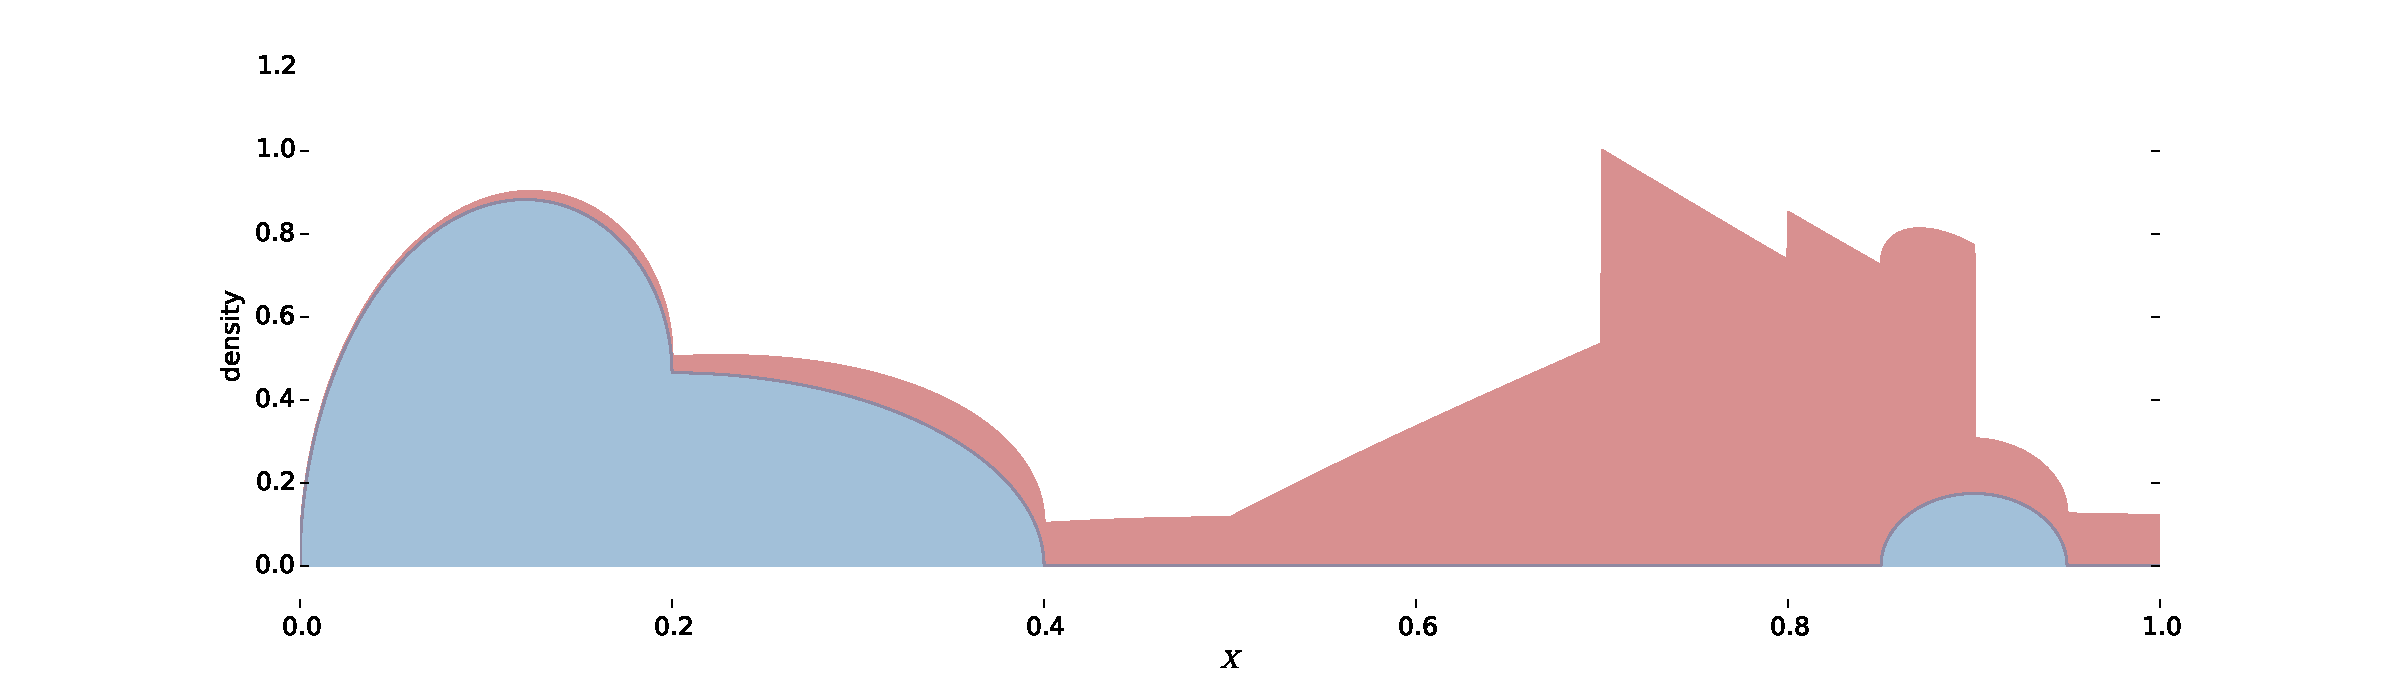
\includegraphics[clip,trim=3cm 0cm 2cm 0cm]{GF/GFgrowth2_profile1d_t0}
}%
\caption{Initial state (blue) $p_0^a$ (red)$p_0^b$}\label{fig_GFWF2_input}
\end{subfigure}
 \begin{subfigure}{.49\linewidth}
\centering
 \resizebox{1.\linewidth}{!}{
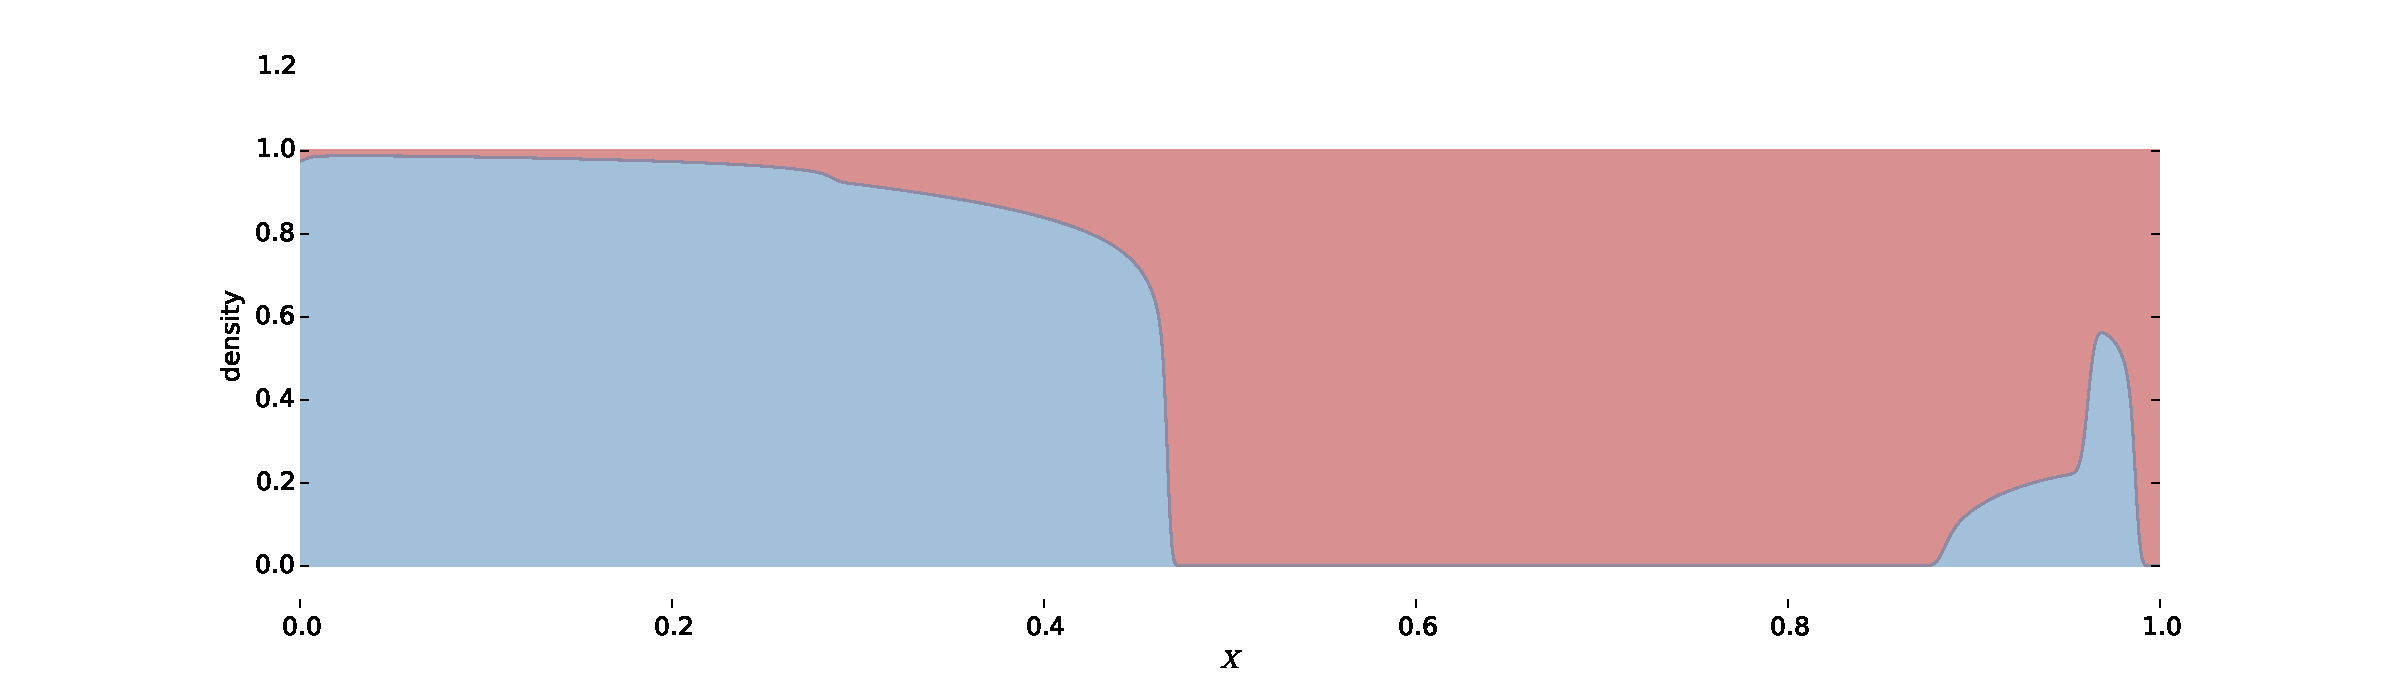
\includegraphics[clip,trim=2cm 0cm 3cm 0cm]{GF/GFgrowth2_profile1d_end}
}
\caption{Steady state densities (for $t$ big)}
\end{subfigure}
\begin{subfigure}{.49\linewidth}
\centering
 \resizebox{.09\linewidth}{!}{
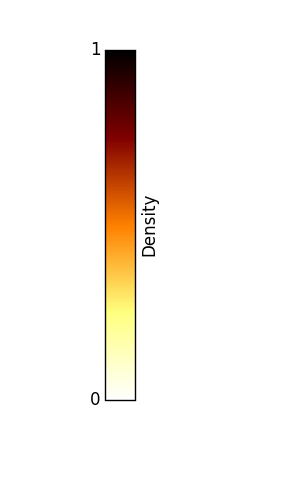
\includegraphics[clip,trim=2cm -2cm 1cm 3cm]{GF/cmapbary}
}%
 \resizebox{.9\linewidth}{!}{
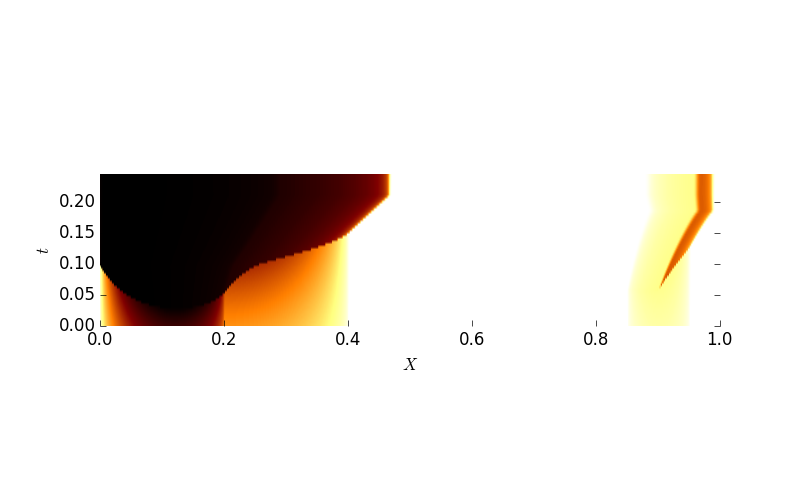
\includegraphics[clip,trim=1.5cm 3cm 1cm 3cm]{GF/GFgrowth2_1d_topa}
}%
\caption{Evolution of $p^a$}
\end{subfigure}
 \begin{subfigure}{.49\linewidth}
\centering
 \resizebox{.9\linewidth}{!}{
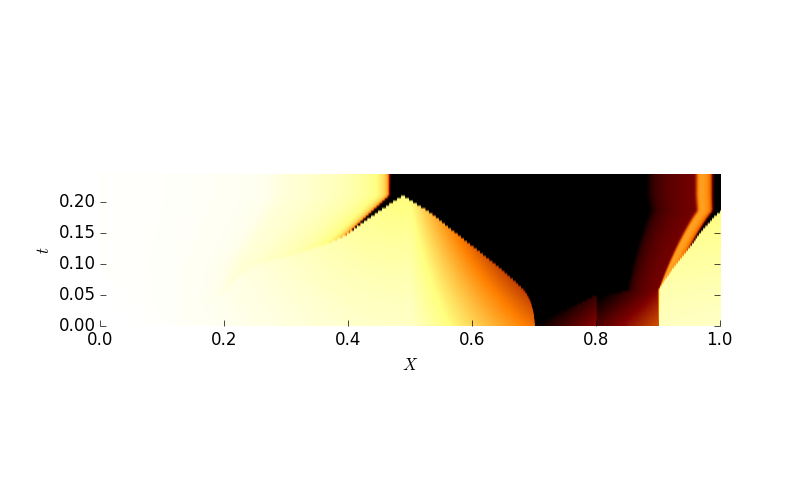
\includegraphics[clip,trim=1cm 3cm 1.5cm 3cm]{GF/GFgrowth2_1d_topb}
}%
 \resizebox{.09\linewidth}{!}{
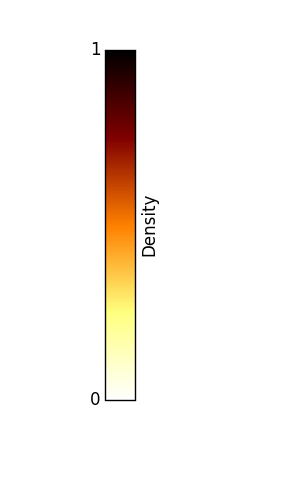
\includegraphics[clip,trim=2cm -2cm 1cm 3cm]{GF/cmapbary}
}
\caption{Evolution of $p^b$}
\end{subfigure}
\caption{(top row) initial state and steady state (density $p^b$ is layered over $p^a$) (bottom row) time evolution (time evolves from bottom to top) with density in color scale.}
\label{fig_WFGF2}
\end{figure}

